\newcommand{\orbital}[3]{#1 \mathrm{#2}_{#3}}

Ústředním úkolem kvantové chemie po zavedení Bornovy-Oppenheimerovy aproximace je výpočet elektronové energie molekul

\begin{equation}
\hat{H}_e \psi_e (\vec{r}, \vec{R}) = E_e (\vec{R}) \psi_e(\vec{r}, \vec{R}),
\label{rov:ElStrukt-1}
\end{equation}

\noindent kde elektronová energie závisí na konkrétní geometrii molekuly, tj. na souřadnicích atomových jader $\vec{R}$. V~této kapitole probereme řešení rovnice \eqref{rov:ElStrukt-1} pro dvouatomové molekuly. Začneme přitom nejjednodušší molekulou, totiž iontem molekuly vodíku H$_2^+$.   

\subsection{Ion molekuly vodíku}

\begin{figure} [htb]
\centering
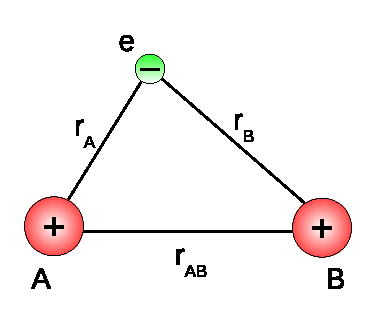
\includegraphics[scale=1]{IonVodiku.eps}
\caption[Ion H$_2^{+}$]{Geometrie iontu molekuly vodíku.}
\label{obr:IonVodiku}
\end{figure}

Ion molekuly vodíku je tvořen dvěma jádry (konkrétně protony), označme si je jako jádra A a~B a jedním elektronem, viz obrázek~\ref{obr:IonVodiku}. Pro takovýto útvar nám není zatěžko napsat elektronový hamiltonián

\begin{equation}
\hat{H}_e = -\frac{\hbar^2}{2 m_e} \Delta_e - \frac{e^2}{4 \pi \epsilon_0} \left( \frac{1}{r_A} + \frac{1}{r_B} \right),
\label{rov:ElStrukt-2}
\end{equation}


\noindent kde
\begin{equation}
\Delta_e \equiv \frac{\partial^2}{\partial x_e^2} + \frac{\partial^2}{\partial y_e^2} + \frac{\partial^2}{\partial z_e^2}
\nonumber
\end{equation}
je Laplaceův operátor v~souřadnicích elektronu $x_e, y_e, z_e$. $r_A$ je souřadnice elektronu k~jádru A a~$r_B$ je souřadnice elektronu k~jádru B.\footnote{V elektronovém hamiltoniánu může, ale nemusí být přidán člen popisující coulombovské odpuzování mezi jádry $\frac{1}{4 \pi \epsilon_0} \frac{e^2}{r_{AB}}$. Z~pohledu elektronové vlnové funkce totiž tento člen představuje konstantu. Zde mezijadernou repulzi vynecháváme}  Nadále bude poněkud pohodlnější pracovat v~soustavě atomových jednotek, ve kterých $\hbar = m_e=e=4\pi \epsilon = 0$. Hamiltonián pak nabude tvaru

\begin{equation}
\hat{H}_e = -\frac{1}{2}\Delta_e - \left( \frac{1}{r_A} + \frac{1}{r_B} \right).
\label{rov:ElStrukt-3}
\end{equation}

Elektronovou Schr\"odingerovu rovnici s~tímto hamiltoniánem je možné řešit analyticky. Nás ale bude zajímat řešení přibližné, takové, které budeme moci využít i pro složitější molekuly. Můžeme se docela dobře odrazit z~naší znalosti elektronové struktury atomů. Kdybychom měli v~blízkosti elektronu pouze jádro A, pak bychom řešení znali: vlnová funkce by byla dána atomovým orbitalem vodíku $1s_A$. Stejně tak kdyby se elektron pohyboval v~blízkosti jádra B a~jádro A~se v~okolí vůbec nevyskytovalo, pak by exaktním řešením byl orbital $1s_B$. Připomeňme, že atomové orbitaly $1s_A$ a~$1s_B$ jsou matematickými funkcemi souřadnic elektronů, konkrétně

\begin{eqnarray}
1\mathrm{s}_A \equiv k^{3/2} \pi^{-1/2} e^{-k r_A}, \nonumber \\
1\mathrm{s}_B \equiv k^{3/2} \pi^{-1/2} e^{-k r_B}, 
\label{rov:ElStrukt-4}
\end{eqnarray}

\noindent kde pro jádro vodíku o~nábojovém čísle $Z=1$ je $k=1$ (pro elektron v~poli jádra He$^+$ je pak $k=2$ atd.). Pokud obě jádra hodně daleko od sebe, pak přesné řešení bude dáno jako

\begin{equation}
\varphi = c_A 1 \mathrm{s}_A + c_b 1\mathrm{s}_B.
\label{rov:ElStrukt-5}
\end{equation}

Uvažme situaci, kdy se elektron nachází v~blízkosti jádra A. Hodnota vlnové funkce $1s_B$ pak pro velké vzdálenosti $r_{AB}$ bude zanedbatelná a tento elektron je pak v~zásadě popsán orbitalem $1s_A$, chová se tedy jako elektron atomu A. Nebo se elektron nachází v~blízkosti jádra B a pak se chová jako elektron atomu B. My budeme předpokládat, že tuto formu vlnové funkce můžeme použít pro všechny mezi-jaderné vzdálenosti. Výraz \eqref{rov:ElStrukt-5} představuje zkusmou vlnovou funkci ve smyslu variačního principu: tato funkce je závislá na rozvojových koeficientech $c_A$ a $c_B$, které musíme určit minimalizací funkcionálu energie.\footnote{Jako variační parametr můžeme použít také parametr $k$. Ten je spojen s~nábojovým číslem. Je jasné, že pro disociovanou strukturu s~velkou mezijadernou vzdáleností $r_{AB}$ bude optimální hodnota $k=1$, budeme skutečně popisovat dva atomy vodíku. Pokud ale obě jádra přiblížíme na velmi malou vzdálenost, vlnová funkce se bude blížit orbitalu $1s$ iontu atomu helia a tedy $k=2$} Tento tvar vlnové funkce je zárodkem metody označované zkratkou MO-LCAO (z~angl. \textit{Molecular Orbitals - Linear Combination of Atomic Orbitals}). Hledáme totiž vlnovou funkci jednoho elektronu pohybujícího se v~molekule (tedy hledáme tzv. molekulový orbital) ve formě lineární kombinace atomových orbitalů. To je klasický příklad lineárního funkcionálu, který vede k~sekulárním rovnicím, se kterými jsme se již několikráte setkali

\begin{eqnarray}
c_A (H_{AA} - E S_{AA} + c_B (H_{AB} - E S_{AB}) = 0, \nonumber \\
c_A (H_{BA} - E S_{AB} + c_B (H_{BB} - E S_{BB}) = 0,
\label{rov:ElStrukt-6}
\end{eqnarray}

\noindent kde coulombovský integrál $H_{AA}$ a $H_{BB}$, rezonanční integrál $H_{AB}$ a překryvový integrál $S_{AB}$ mají v~našem případě tvar

\begin{eqnarray}
H_{AA} = H_{BB} &=& \frac{1}{2} k^2 - k~- \frac{1}{r_{AB}} - e^{2 k~r_{AB}} \left( k~+ \frac{1}{r_{AB}} \right), \nonumber \\
H_{AB} &=& -\frac{1}{2}k S_{AB} - k~(2-k) (1+ k~r_{AB}) e^{-k r_{AB}}, \nonumber \\
S_{AB} &=& e^{-k r_{AB}} \left(1 + k~r_{AB} + \frac{1}{3}k^2 r_{AB}^2 \right).
\label{rov:ElStrukt-7}
\end{eqnarray}

Podmínkou netriviálního řešení sekulárních rovnic je nulovost sekulárního determinantu


\begin{equation}
\begin{vmatrix}
H_{AA} - E S_{AA} & H_{AB} - E S_{AB}\\
H_{BA} - E S_{AB} & H_{BB} - E S_{AB}
\end{vmatrix}
=0,
\label{rov:ElStrukt-8}
\end{equation}

\noindent což vede k~dvěma možným hodnotám energie (uvažme přitom, že hodnota rezonančního integrálu $H_{AB}$ je záporná)

\begin{eqnarray}
E_1 = \frac{H_{AA} + H_{AB}}{1+S_{AB}}, \nonumber \\
E_2 = \frac{H_{AA} - H_{AB}}{1-S_{AB}}.
\label{rov:ElStrukt-9}
\end{eqnarray}

Jestliže dosadíme energii $E_1$ zpět do sekulárních rovnic (detaily viz příklad \ref{priklad var princip} v kapitole~\ref{kap:Lin Var funkcional}), získáme vztah 

\begin{equation}
c_A = c_B.
\label{rov:ElStrukt-10}
\end{equation}

Pokud do sekulárních rovnic  dosadíme za energii hodnotu $E_2$, získáme vztah

\begin{equation}
c_A = - c_B.
\label{rov:ElStrukt-11}
\end{equation}

\noindent Hodnoty rozvojových koeficientů se tak v~absolutní hodnotě musí rovnat, lišit se může pouze jejich znaménko. To jsme ani nemuseli počítat z~variačního principu, neboť to plyne přímo ze symetrie problému. Máme tak dvojí řešení, pro základní stav s~energií $E_1$ je řešením molekulový orbital jako součet atomových orbitalů

\begin{equation}
\varphi_1 = c_A (1\mathrm{s}_A + 1\mathrm{s}_B).
\label{rov:ElStrukt-12}
\end{equation}

\noindent Mluvíme o~tzv. vazebném orbitalu. Pro excitovaný stav s~energií $E_2$ je řešením Schr\"odingerovy rovnice rozdíl těchto atomových orbitalů

\begin{equation}
\varphi_2 = c_A(1\mathrm{s}_A - 1\mathrm{s}_B).
\label{rov:ElStrukt-13}
\end{equation}

\noindent zde mluvíme o~antivazebném orbitalu. Obrázek \ref{obr:Vodik-orbitaly} vysvětluje toto označení. Ve vazebném orbitalu je maximum elektronové hustoty soustředěno do oblasti mezi atomovými jádry. Takovéto uspořádání podporuje přibližování atomových jader. Na druhou stranu v~antivazebném orbitalu elektrony mezi jádry příliš nejsou a obě jádra se tak od sebe odpuzují. \footnote{Obrázek by mohl vzbuzovat dojem, že primární hnací silou chemické vazby je elektrostatické stínění odpudivé interakce mezi jádry. To je ale přinejmenším nepřesné. Hlavním tahounem poklesu energie při vzniku vazby je pokles kinetické energie elektronů.} 

\begin{figure} [htb]
\centering
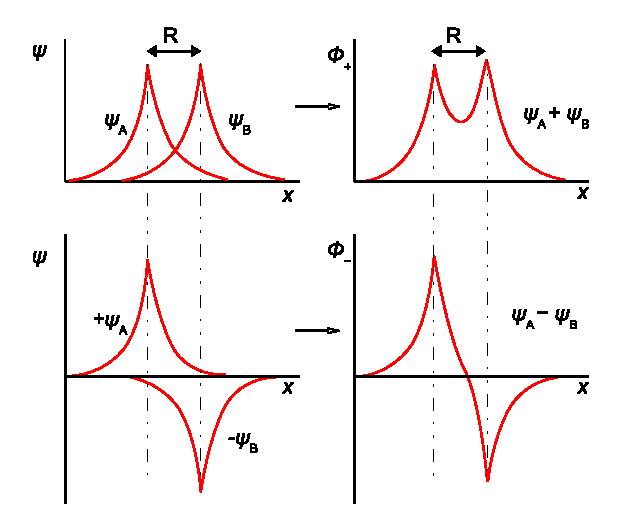
\includegraphics[scale=1]{Orbitaly.eps}
\caption[Orbitaly iontu vodíku]{Vazebný a antivazebný orbital iontu molekuly vodíku.}
\label{obr:Vodik-orbitaly}
\end{figure}

\begin{figure} [htb]
\centering
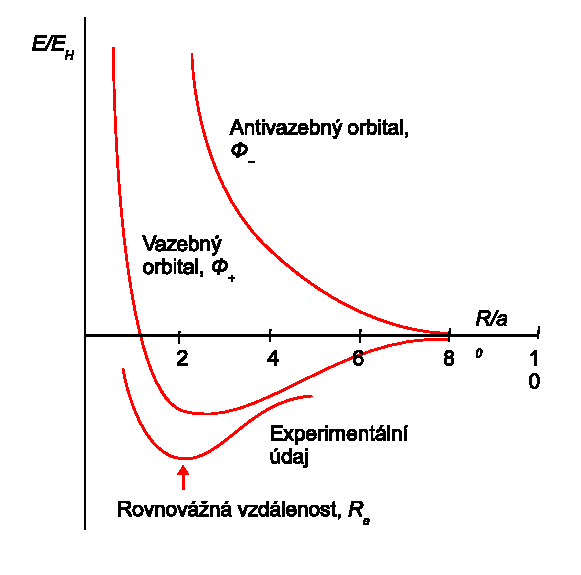
\includegraphics[scale=1]{PotencialovaKrivka.eps}
\caption[Potenciálové křivky iontu vodíku]{Potenciálové křivky dvou nejnižších stavů iontu molekuly vodíku.}
\label{obr:PotencialovaKrivka}
\end{figure}

\noindent Z~rovnice \eqref{rov:ElStrukt-7} můžeme do grafu snadno vynést energie $E_1$ a $E_2$ v~závislosti na mezijaderné vzdálenosti $r_{AB}$. Přidáme-li ještě mezijadernou repulzi $1/r_{AB}$, získáme křivky zobrazené na obrázek~\ref{obr:Vodik-orbitaly}.

Pro úplnost zbývá ještě doplnit, že konkrétní hodnotu rozvojového koeficientu $c_A$ získáme z~normalizačních podmínek


\begin{eqnarray}
1 &=& \int \vert \varphi_1 \vert^2 \mathrm{d}\tau = c_A^2 \int (1\mathrm{s}_A^2 + 1 \mathrm{s}_B^2 + 2 \cdot 1\mathrm{s}_A 1\mathrm{s}_B) \mathrm{d}\tau = c_A^2 (2 + 2S_{AB}), \nonumber \\
1 &=& \int \vert \varphi_2 \vert^2 \mathrm{d}\tau = c_A^2 \int (1\mathrm{s}_A^2 + 1 \mathrm{s}_B^2 - 2 \cdot 1\mathrm{s}_A 1\mathrm{s}_B) \mathrm{d}\tau = c_A^2 (2 - 2S_{AB}) 
\label{rov:ElStrukt-14}
\end{eqnarray}


\noindent a vlnová funkce tak má tvar


\begin{eqnarray}
\phi_1 &=& \frac{1\mathrm{s}_A + 1\mathrm{s}_B}{\sqrt{2}(1+S_{AB})}, \nonumber \\
\phi_2 &=& \frac{1\mathrm{s}_A - 1\mathrm{s}_B}{\sqrt{2}(1-S_{AB})}
\label{rov:ElStrukt-15}
\end{eqnarray}

\subsection{Molekulové orbitaly excitovaných stavů}

Výpočet elektronové energie iontu molekuly vodíku představený v~minulé kapitole je pouze velmi přibližný. Jak bychom jej mohli vylepšit? Jedna z~možností by byla považovat $k$ v~\eqref{rov:ElStrukt-4} za variační parametr. To je ale matematicky poněkud obtížnější úkol, neměli bychom pak již lineární funkcionál. Jinou, fyzikálně dobře motivovanou, možností je rozvinout molekulové orbitaly do rozsáhlejší množiny atomových orbitalů, například uvažovat elektron pohybující se ne pouze v~základním stavu atomu vodíku, ale i v~jeho stavech excitovaných. Mohli bychom například psát

\begin{eqnarray}
\varphi &=& c_1 \orbital{1}{s}{A} + c_2 \orbital{1}{s}{b} + c_3 \orbital{2}{s}{A} + c_4 \orbital{2}{s}{B} + \nonumber \\
&+& c_5 \orbital{2}{(p_1)}{A} + c_6 \orbital{2}{(p_1)}{B} + c_7 \orbital{2}{(p_0)}{A} + c_8 \orbital{2}{(p_0)}{B} + c_9 \orbital{2}{(p_{-1})}{A} + c_{10} \orbital{2}{(p_{-1})}{B}.
\label{rov:ElStrukt-16}
\end{eqnarray}

\noindent Takovýto rozvoj zvýší flexibilitu vlnové funkce. Sekulární rovnice nyní již představují soustavu deseti rovnic pro deset neznámých rozvojových koeficientů. Pořád ale jde o~soustavu lineárních rovnic, které jsou snadno řešitelné. Na místo dvou stavů ale nyní získáme stavů deset. V~základním stavu získáme řešením funkci, jejímž dominantním členem bude součet $1s_A+1s_B$, ale v~určité malé míře budou k~řešení přispívat i orbitalu $2s_A$, $(2p_0)_A$, $2s_B$ či $(2p_0)_A$, v~excitovaných stavech se začnou výrazněji uplatňovat i vyšší atomové orbitaly. Při kombinování atomových orbitalů do orbitalů molekulových bude platit

\begin{itemize}
\item V~jednom molekulovém orbitalu se budou výrazněji uplatňovat pouze atomové orbitaly o~podobné energii. To vyplývá jednak z~matematiky celého problému, jednak i ze selského rozumu. Jestliže se elektron v~atomu A~pohybuje s~určitou energií, nemůžeme asi čekat, že se v~blízkosti atomu B jeho energie závratně změní.

\item Kombinují se toliko atomové orbitaly o~stejné symetrii vůči prvkům symetrie dané molekuly. Nebude se tak kombinovat orbital $1s_A$ s~orbitalem $(2p_1)_B$, neboť tyto orbitaly mají nulový překryv. Díky tomu můžeme řešit zvlášť sekulární problém pro $\sigma$ a $\pi$ elektrony

\begin{eqnarray}
\varphi_{\sigma} &=& c_1 \orbital{1}{s}{A} + c_2 \orbital{1}{s}{B} + c_3 \orbital{
2}{s}{A} + c_4 \orbital{2}{s}{B} + c_5 \orbital{2}{(p_0)}{A} + c_6 \orbital{2}{(p_0)}{B}, \nonumber \\
\varphi_{\pi} &=& c_1 \orbital{2}{(p_1)}{A} + c_2 \orbital{2}{(p_1)}{B} + c_3 \orbital{
2}{(p_{-1})}{A} + c_4 \orbital{2}{(p_{-1})}{B}.
\label{rov:ElStrukt-17}
\end{eqnarray}

\end{itemize}


\subsection{Více-elektronové molekuly}
Není asi snadné nadchnout chemika pro otázky spojené s~iontem molekuly vodíku. Skutečně, skoro vše, co chemika zajímá, má elektronů více. Mohou nám nějak výše uvedené úvahy pomoci při řešení otázek spojenými s~více-elektronovými molekulami? Ano, může. V~rámci Hartreeho-Fockovy aproximace totiž $N$-elektronovou Schr\"odingerovu rovnici 

\begin{equation}
\hat{H} \psi (\vec{r_1}, \vec{r_2}, \dots \vec{r_N}) = E_e\psi (\vec{r_1}, \vec{r_2}, \dots \vec{r_N})
\label{rov:ElStrukt-18}
\end{equation}

\noindent redukujeme na $N$ jednoelektronových Fockových rovnic pro jednotlivé elektrony

\begin{equation}
\hat{F}_i \phi_i (\vec{r_i}) = \varepsilon_i \phi_i (\vec{r_i}).
\label{rov:ElStrukt-19}
\end{equation}

\noindent Fockovy rovnice obsahují složitější operátor než ten, se kterým jsme se setkali při řešení iontu molekuly vodíku, vše co bylo řečeno ale platí i pro molekulové orbitaly více-elektronových molekul. Stále tak hledáme molekulové orbitaly $\phi$ jako lineární kombinace atomových orbitalů $\chi_j$

\begin{equation}
\varphi_i(\vec{r_i}) = \sum_i c_{ji} \chi_j (\vec{r_i}),
\label{rov:ElStrukt-20}
\end{equation}

\noindent přičemž rozvojové koeficienty $c_{ji}$ získáváme pomocí variačního principu. Výsledky takovýchto výpočtů jsou důvěrně známé každému pečlivějšímu čtenáři základních učebnic anorganické chemie. Uplatňují se přitom dvě výše zmíněná pravidla o~kombinování orbitalů. Není cílem této přednášky dopodrobna opakovat celý tak důvěrně známý příběh. Pro připomenutí však čtenáře odkazujeme na obrázku~\ref{obr:Diatomy} zobrazující elektronové hladiny v~homonuklárních diatomických molekulách.

\begin{figure} [htb]
\centering
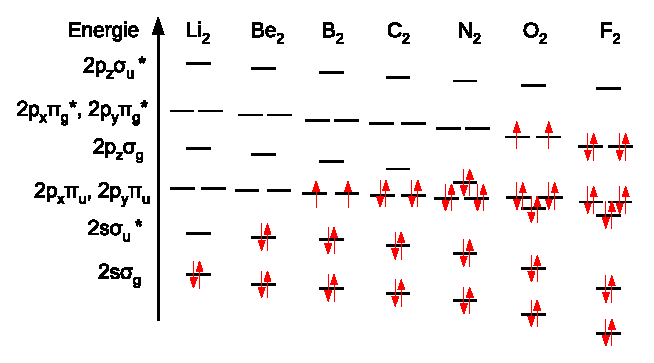
\includegraphics[scale=1]{Diatomy.eps}
\caption[Diatomické molekuly]{Jednoelektronové stavy v homonukleárních diatomických molekulách.}
\label{obr:Diatomy}
\end{figure}

Připomeňme také, že s~výše uvedenými orbitálními diagramy je spojen pojem řád vazby, definovaný jako

\begin{equation}
BO = \frac{n_r - n^{\ast}}{2}
\label{rov:ElStrukt-21}
\end{equation}

\noindent který nám říká, \uv{kolikatinásobná} je příslušná vazba. Číslo $n_r$ je počet elektronů ve vazebných orbitalech a $n^{\ast}$ je počet elektronů v~antivazebných orbitalech. Tak například vidíme, že molekula dusíku je vázána trojnásobnou vazbou. Taktéž by nám neměla uniknout překvapivá prediktivní síla kvalitativní teorie molekulových orbitalů. Z~diagramu pro molekulu O$_2$ kupříkladu hned vidíme, že tato molekula by měla být paramagnetická, neboť představuje dle Hundova pravidla biradikál, má totiž dva nepárové elektrony.

Zatím jsme se dívali pouze na diatomické molekuly tvořené dvěma stejnými atomy (homonukleární diatomika. Nic nám ale nebrání hledat molekulové orbitaly popisující pohyb elektronů v~diatomickcýh molekulách s~nestejnými atomy. Podívejme se na případ molekuly NO. energie 2p orbitalu atomu dusíku je -15~eV, energie 2p orbitalu atomu kyslíku je -17~eV. Orbitální diagram pak vypadá takto

\begin{figure} [htb]
\centering
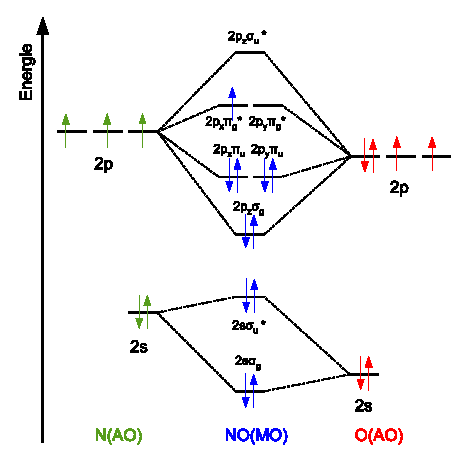
\includegraphics[scale=1]{NO-orbitaly.eps}
\caption[Orbitaly NO]{Orbitální diagram molekuly NO. Znázorněny jsou interakce pouze 2p a 2s orbitalů.}
\label{obr:NO-orbitaly}
\end{figure}

\noindent Jelikož je energie atomu dusíku nižší, budou MO vazebných orbitalů tvořeny z~větší míry právě orbitaly atomu N a na tom tak bude soustředěn větší záporný náboj. Všimněme si také, že molekula NO představuje dle tohoto schématu radikál.


Podívejme se ještě na jeden případ, na molekulu fluorovodíku. Elektron v~1s orbitalu atomu vodíku má energii -13,6 eV, elektron v~2p orbitalu atomu fluoru má hodnotu -17,4 eV. Orbitální diagram pak bude vypadat takto

\begin{figure} [htb]
\centering
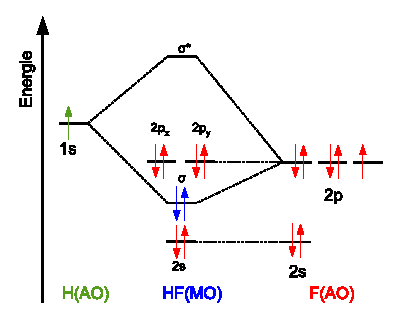
\includegraphics[scale=1]{HF-orbitaly.eps}
\caption[Orbitaly HF]{Orbitální diagram molekuly HF.}
\label{obr:HF-orbitaly}
\end{figure}

\noindent S~1s orbitalem atomu vodíku se ze symetrických důvodů může kombinovat pouze jediný z~2p orbitalů atomu fluoru. Zbylé dva orbitaly se vazby neúčastní, nejsou vazebné, ani antivazebné, nýbrž nevazebné. Opět vidíme, že vazebný orbital bude mít větší příspěvek  od atomu fluoru, konkrétně

\begin{equation}
\varphi_1 = 0{,}34 \cdot \orbital{1}{s}{\mathrm{H}} + 0{,}84 \cdot \orbital{2}{p_z}{\mathrm{F}}
\label{rov:ElStrukt-22}
\end{equation}


\noindent naopak antivazebný orbital bude mít větší příspěvek od atomu vodíku

\begin{equation}
\varphi_2 = 0{,}44 \cdot \orbital{1}{s}{\mathrm{H}} - 0{,}63 \cdot \orbital{2}{p_z}{\mathrm{F}},
\label{rov:ElStrukt-23}
\end{equation}


\noindent jelikož v~základním stavu elektrony nevazebný orbital nezaplňují, bude větší elektronová hustota lokalizovaná na atomu fluoru a ten tak bude mít záporný parciální náboj. Tento typ úvah je základem tzv. Mullikenovy populační analýzy, o~které na přednášce bude řeč ještě později.


Na závěr tohoto oddílu si ještě zopakujme, jakým způsobem přistupujeme k~řešení $N$-elektronovou Schr\"odingerovy rovnice v~rámci přístupu MO-LCAO. Předpokládáme, že známe řešení pro orbitaly atomů vodíkového typu (tyto funkce přitom mohou obsahovat určité variační parametry). Jejich uspořádáním do Slaterova determinantu vytvoříme mnohaelektronovou vlnovou funkci a v~rámci metody Hartreeho-Focka tak vypočítáme elektronovou energii atomů. Jednoelektronové vlnové funkce atomů vodíkového typu můžeme v~rámci přístupu MO-LCAO zkombinovat do molekulových orbitalů, ze kterých pak vytvoříme opět mnohaelektronovou vlnovou funkci uspořádáním do Slaterova determinantu, viz. obrázek~\ref{obr:MOLCAO}.

\begin{figure} [htb]
\centering
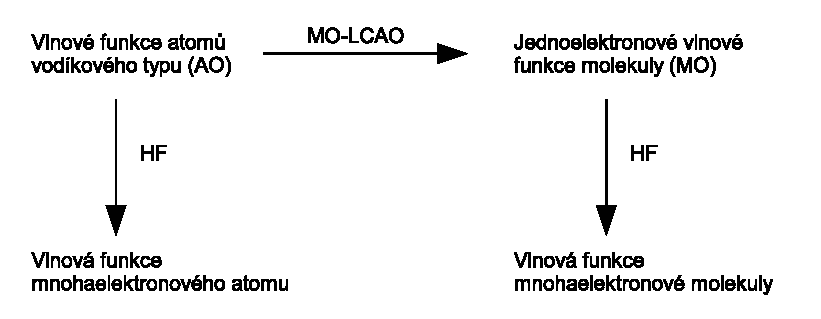
\includegraphics[scale=1]{Metoda-MO-LCAO.eps}
\caption{Metoda MO-LCAO}
\label{obr:MOLCAO}
\end{figure}


\subsection{Klasifikace molekulových orbitalů a elektronové termy dvouatomových molekul}
 
Jednoelektronové vlnové funkce molekul, tj. molekulové orbitaly, můžeme klasifikovat s~ohledem na chování vlnové funkce vůči prvkům symetrie molekul. Všechny diatomické molekuly mají nekonečně četnou osu symetrie $C_\infty$. Homonukleární diatomika mají navíc střed symetrie.

Z~hlediska chování vlnové funkce vůči ose symetrie $C_\infty$ mluvíme o 

\begin{itemize}

\item Orbitalu $\sigma$, jestliže rotace kolem osy $C_\infty$ ponechá orbital nezměněn.

\item Orbitalu $\pi$, jestliže je osa $C_\infty$ obsažena v~jedné uzlové rovině (tj. v~rovině, ve které je hodnota vlnové funkce nulová)

\item Orbitalu $\delta$, jestliže je osa $C_\infty$ obsažena ve dvou uzlových rovinách. 

\end{itemize}

\noindent A~takto bychom mohli pokračovat dále. Z~hlediska středu symetrie můžeme orbitaly klasifikovat jako 

\begin{itemize}

\item g (údajně z~něm. \textit{gerade}), kdy operace zrcadlení dle středu symetrie nemění znaménko vlnové funkce

\item u~(údajně z~něm. \textit{ungerade}), kdy operace zrcadlení dle středu symetrie mění znaménko vlnové funkce 

\end{itemize}

Na obrázku~\ref{obr:KlasifikaceMO} je klasifikace orbitalů znázorněna na několika příkladech.

\begin{figure} [htb]
\centering
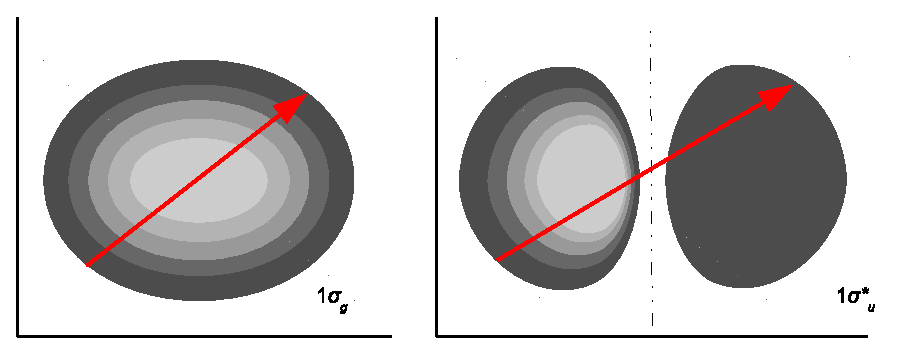
\includegraphics[scale=.8]{KlasOrbitaly.eps}
\caption[Klasifikace MO]{Příklad klasifikace molekulových orbitalů.}
\label{obr:KlasifikaceMO}
\end{figure}
 

Pojďme se ještě zamyslet nad otázkou, zda klasifikace dle orbitalů dle symetrie nemá ještě nějaký hlubší význam. Symetrie je obvykle znakem zachování určité fyzikální veličiny. U~molekul už nemůžeme předpokládat zachování momentu hybnosti jako u~atomů, neboť elektrony v~molekulách se nepohybují v~centrálním poli. Molekuly mají pořád ještě válcovou symetrii a~zachovává se tak průmět momentu hybnosti do osy $z$, $L_z$. Zavedeme-li si nyní kvantové číslo $\lambda= |m|$, kde $m=0,+-1,+-2$ atd., můžeme udělat následující přiřazení


\begin{table} [htb]
\centering
\begin{tabular}{c|c|c|c|c|c}
\toprule
$\lambda$ & 0 & 1 & 2 & 3 & 4\\
\midrule
označení & $\sigma$ & $\pi$ & $\delta$ & $\phi$ & $\gamma$\\
\bottomrule
\end{tabular}
\end{table}


Ve vícelektronových molekulách se moment hybnosti ve směru osy $z$ může sčítat. Celkové magnetické kvantové číslo $M_L$ vícelektronové molekuly je pak dáno prostým součtem magnetických kvantových čísel $m$ jednotlivých elektronů. Zavádíme pak kvantové číslo 

\begin{equation}
\Lambda = \vert M_L \vert
\label{rov:ElStrukt-24}
\end{equation}   
      
\noindent a opět zavádíme značení


\begin{table} [H]
\centering
\begin{tabular}{c|c|c|c|c|c}
\toprule
$\Lambda$ & 0 & 1 & 2 & 3 & 4\\
\midrule
označení & $\Sigma$ & $\Pi$ & $\Delta$ & $\Phi$ & $\Gamma$\\
\bottomrule
\end{tabular}
\end{table}

\begin{priklad}
\textbf{Zadání A:} Mějme konfiguraci $\sigma\sigma$. Určete možné stavy této molekuly.\\[0.1cm]
\textbf{Řešení A:} 
\begin{displaymath}
^{1}\Sigma, \, ^{3}\Sigma.
\end{displaymath}

\textbf{Zadání B:} Mějme konfiguraci $\pi\pi$. Určete možné stavy této molekuly.\\[0.1cm]
\textbf{Řešení B:}
\begin{displaymath}
^{1}\Sigma, \, ^{3}\Sigma, \, ^{1}\Delta, \, ^{3}\Delta.
\end{displaymath} \vspace{-0.7cm}
\end{priklad}

Můžeme pak ještě uvažovat celkový moment hybnosti $\vec{\Omega}$ daný součtem orbitálního a spinového momentu molekuly. Odpovídající kvantové číslo nabývá hodnot

\begin{equation}
\Lambda + S, \, \Lambda + S - 1, \dots, \Lambda - S. 
\label{rov:ElStrukt-25}
\end{equation}

\begin{priklad}
\textbf{Zadání:} V~jakých stavech se může nacházet molekula ve stavu $^4\Pi$?\\[0.1cm]
\textbf{Řešení:}
\begin{displaymath}
^4\Pi_{5/2}, \, ^4\Pi_{3/2}, \, ^4\Pi_{1/2}, \, ^4\Pi_{-1/2}.
\end{displaymath} \vspace{-0.7cm}
\end{priklad}

Energetické rozštěpení těchto stavů je pro prvky o~malém protonovém čísle velmi malé, je dáno pouze spin-orbitální interakcí, o~které již byla řeč dříve. 


\subsection{Molekulové orbitaly víceatomových molekul}
Doposud jsme diskutovali pouze diatomické molekuly. Elektronovou energii můžeme ale prostřednictvím Hartreeho-Fockovy metody stejně dobře hledat i pro molekuly víceatomové. Opět budeme hledat molekulové orbitaly jako lineární kombinaci atomových orbitalů. Tyto molekulové orbitaly nemůžeme již klasifikovat s~ohledem na chování vůči ose symetrie $C_\infty$, neboť obecně molekuly takovouto symetrii nevykazují. I~nižší symetrie ale mohou sloužit k~označování molekulových orbitalů. Příklad molekulových orbitalů víceatomové molekuly lze najít na obrázku~\ref{obr:Voda_Orbitaly}.

\begin{figure} [htb]
\centering
\includegraphics[scale=.8]{Voda_Orbitaly.eps}
\caption{Molekulové orbitaly molekuly vody.}
\label{obr:Voda_Orbitaly}
\end{figure}

 
Všimněme si, že v~případě molekuly vody není tak úplně snadné říci, zda je o~orbital vazebný či antivazebný. Příslušné molekulové orbitaly jsou totiž delokalizovány přes celou molekulu. Rozhodně se nedá říci, že určitý molekulový orbital náležel určité vazbě. Pro chemika to není úplně komfortní situace. Od dob Lewisových je zvyklý si chemickou vazbu představovat jako sdílený elektronový pár. Tento pár by se pak dle chemického pohledu měl nacházet někde mezi dvěma atomy, jako je tou v~případě diatomických molekul. 

Tomuto pohledu v~principu není obtížné vyjít vstříc. Orbitaly jsou totiž pouze pomocnými veličinami, fyzikálně pozorovatelné veličiny závisí toliko na celkové vlnové funkci. Každá transformace orbitalu taková, že zanechá vlnovou funkci až na znaménko netknutou je proto možná. Jak taková povolená transformace má vypadat? Zaveďme si tzv. unitární matici vztahem

\begin{equation}
\mathbf{U}^{\ast} \mathbf{U} = \mathbf{1}.
\label{rov:ElStrukt-26}
\end{equation}

\noindent Potom bude nutně platit

\begin{equation}
\mbox{det} \vert \mathbf{U}^{\ast} \vert \cdot \mbox{det} \vert \mathbf{U} \vert = \mathbf{1}.
\label{rov:ElStrukt-27}
\end{equation}

\noindent Z~čehož ale vyplývá, že 

\begin{eqnarray}
\mbox{det} \vert \mathbf{U} \vert &=& e^{i\lambda}, \nonumber \\
\mbox{det} \vert \mathbf{U}^{\ast} \vert &=& e^{-i\lambda},
\label{rov:ElStrukt-28}
\end{eqnarray}


\noindent kde $\lambda$ je libovolné číslo. Nyní si definujme matici 


\begin{equation}
\mathbf{A}=
\begin{pmatrix}
\phi_1(1) & \phi_1(2) & \ldots & \phi_1(N) \\
\vdots & \vdots & & \vdots \\
\phi_N(1) & \phi_N (2) & \ldots & \phi_N(N)
\end{pmatrix}.
\label{rov:ElStrukt-29}
\end{equation}


\noindent Harteeho-Fockova vlnová funkce je pak dána jako


\begin{equation}
\psi(1,2, \dots, N) = \mbox{det} \mathbf{A}.
\label{rov:ElStrukt-30}
\end{equation}


\noindent Mějme nyní transformovanou sadu orbitalů


\begin{equation}
\begin{pmatrix}
\phi_1^{\prime} \\
\vdots \\
\phi_N^{\prime}
\end{pmatrix}
= \mathbf{U} 
\begin{pmatrix}
\phi_1 \\
\vdots \\
\phi_N
\end{pmatrix}.
\label{rov:ElStrukt-31}
\end{equation}


\noindent A~v~této sadě napišme Slaterův determinant

\begin{equation}
\psi^{\prime}(1,2, \dots, N) = \mbox{det} ( \mathbf{U} \cdot \mathbf{A}).
\label{rov:ElStrukt-32}
\end{equation}

\noindent Z~čehož 

\begin{equation}
\psi^{\prime}(1,2, \dots, N) = e^{i \lambda} \psi(1,2, \dots, N).
\label{rov:ElStrukt-33}
\end{equation}

\noindent Pro reálné vlnové funkce faktor $e^{i\lambda}$  neznamená než změnu znaménka. Vidíme tedy, že jakákoliv unitární transformace orbitalů nevede k~závažné změně vlnové funkce. Transformovaná sada orbitalů je stejně dobrou sadou jako ta původní. Nikdo nám proto nemůže zabránit ve vytvoření sady atomových orbitalů, která v~případě tetraedrického uspořádání vazeb jako v~případě molekuly vody poveden ke čtyřem orbitalům mířícím do vrcholu tetraedru


\begin{eqnarray}
\phi^{\prime}_1 &=& \frac{1}{2} ( 2 \mathrm{s} + 2 \mathrm{p_x} + 2 \mathrm{p_y} + 2 \mathrm{p_z}) \quad \phi^{\prime}_3 = \frac{1}{2} ( 2 \mathrm{s} + 2 \mathrm{p_x} - 2 \mathrm{p_y} - 2 \mathrm{p_z}), \nonumber \\
\phi^{\prime}_2 &=& \frac{1}{2} ( 2 \mathrm{s} - 2 \mathrm{p_x} - 2 \mathrm{p_y} + 2 \mathrm{p_z}) \quad \phi^{\prime}_4 = \frac{1}{2} ( 2 \mathrm{s} - 2 \mathrm{p_x} + 2 \mathrm{p_y} - 2 \mathrm{p_z}).
\label{rov:ElStrukt-34}
\end{eqnarray}


Tyto tzv. \textbf{hybridní orbitaly} je možné využít ke konstrukci molekulových orbitalů molekuly vody (či kupříkladu molekuly methanu). Získané orbitaly se budou nacházet v~oblasti vazeb. Jde ale o~změnu víceméně kosmetickou a není žádoucí pojem hybridizace přeceňovat. Poznamenejme, že původní, tzv. kanonické, orbitaly jsou v~jistém smyslu \uv{fyzikálnější}, neboť pouze pro ně (a nikoliv pro hybridní orbitaly) platí Koopmansův teorém.\footnote{K diskuzi o~hybridních orbitalech odkazujeme na starší článek A. Sadleje a R. Zahradníka \textit{Jsou chemické jevy podmíněné hybridizací?} Chem. Listy \textbf{1981}, 75, 561-562, stejně jako na nedávnou zajímavou výměnu názorů iniciovanou textem A. Grushowa \textit{\uv{Is It Time To Retire the Hybrid Atomic Orbital?}} J. Chem. Educ. \textbf{2011}, 88, 860-862 } Pro případ orbitalů \eqref{rov:ElStrukt-34} má matice $\mathbf{U}$ tvar

\begin{equation}
\mathbf{U} = 
\begin{pmatrix}
1 & 1 & 1 & 1 \\
1 & -1 & -1 & 1 \\
1 & 1 & -1 & -1\\
1 & -1 & 1 & -1
\end{pmatrix}.
\end{equation}

\noindent Snadno se přesvědčíme, že matice je skutečně unitární.


        
   



      





